\documentclass{article}
\usepackage[margin=1in]{geometry}
\usepackage{amsmath,amsthm,amssymb}
\usepackage{bbm,enumerate,mathtools}
\usepackage{tikz,pgfplots}
\usepackage{chessboard}
\usepackage[hidelinks]{hyperref}
\usepackage{multicol} % Problem 35

\newenvironment{question}{\begin{trivlist}\item[\textbf{Question.}]}{\end{trivlist}}
\newenvironment{note}{\begin{trivlist}\item[\textbf{Note.}]}{\end{trivlist}}
\newenvironment{references}{\begin{trivlist}\item[\textbf{References.}]}{\end{trivlist}}
\newenvironment{related}{\begin{trivlist}\item[\textbf{Related.}]\end{trivlist}\begin{enumerate}}{\end{enumerate}}


\begin{document}
\rating{4}{2}
Consider partitions of the $n \times m$ grid in which every piece has
$180^\circ$ rotational symmetry.
\begin{figure}[!h]
  \centering
  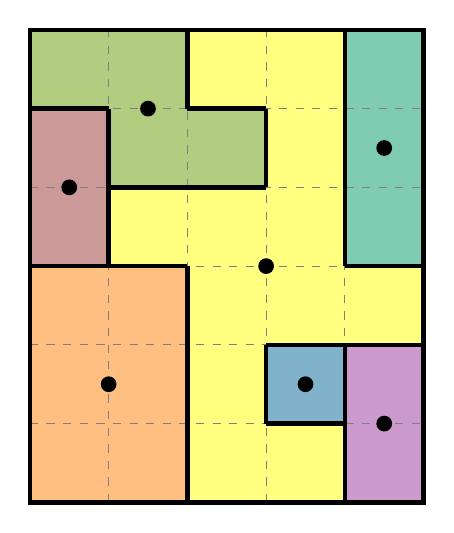
\begin{tikzpicture}

    \fill[fill={rgb:white,1;yellow,1}]             (0, 0) rectangle (5, 6);
    \fill[fill={rgb:white,4;red,2;yellow,2}]       (0, 0) rectangle (2, 3);
    \fill[fill={rgb:white,5;red,3;green,1;blue,1}] (0, 3) rectangle (1, 5);
    \fill[fill={rgb:white,5;red,2;green,3}]        (0, 5) rectangle (2, 6); \fill[fill={rgb:white,5;red,2;green,3}] (1, 4) rectangle (3, 5);
    \fill[fill={rgb:white,5;red,2;blue,3}]         (4, 0) rectangle (5, 1);
    \fill[fill={rgb:white,3;red,1;blue,1}]         (4, 0) rectangle (5, 2);
    \fill[fill={rgb:white,5;green,2;blue,3}]       (3, 1) rectangle (4, 2);
    \fill[fill={rgb:white,5;green,3;blue,2}]       (4, 3) rectangle (5, 6);

    \draw[gray, dashed] (0,0) grid (5,6);
    \draw[ultra thick] (0, 0) rectangle (5, 6);

    \def\lines{
      0/5/1/5, 2/5/3/5, 1/4/3/4, 0/3/2/3, 4/3/5/3, 3/2/5/2, 3/1/4/1,
      1/3/1/5, 2/0/2/3, 2/5/2/6, 3/1/3/2, 3/4/3/5, 4/0/4/2, 4/3/4/6
    }
    \foreach \a/\b/\x/\y in \lines {
      \draw[ultra thick] (\a, \b)--(\x,\y);
    }

    \def\centers{
      0.5/4, 1/1.5, 1.5/5, 3/3, 3.5/1.5, 4.5/1, 4.5/4.5
    }
    \foreach \x/\y in \centers {
      \fill (\x, \y) circle (0.1cm);
    }
  \end{tikzpicture}
  \caption{A partition of the $5 \times 6$ grid into $7$ parts with rotational symmetry.}
\end{figure}

\begin{question}
  How many such partitions of the $n \times n$ grid exist? Up to dihedral action?
\end{question}
\begin{related}
  \item How many partitions into exactly $k$ parts?
  \item How many partitions with other types of symmetry?
  \item How many partitions of a torus? Cylinder? M\"obius strip?
  \item How many partitions of a triangular or hexagonal lattice?
  \item How many partitions of an $n \times m \times p$ cuboid?
\end{related}
\begin{references}
  \item \url{https://www.chiark.greenend.org.uk/~sgtatham/puzzles/js/galaxies.html}
\end{references}
\end{document}
